\documentclass{report}

% packages without any option
\usepackage
{
  graphicx,
  listings,
}

% packages with options
\usepackage[svgnames]{xcolor}
\usepackage[a4paper]{geometry}
\usepackage[document]{ragged2e}

% preamble
\title{BSMRSTU Multimedia Player}
\author{Md. Kazi Iqbal Hossen \& Rafiqur Rahman Ripon}
\date{\today}

% configuration
\lstset
{
 language = Java,
 backgroundcolor = \color{black!5},
 basicstyle = \footnotesize\ttfamily, % Add all style properties without comma separator.
 keywordstyle = \color{blue},
 commentstyle = \color{gray!90},
 showstringspaces = false,
 stringstyle = \color{green},
 captionpos = b %, b: bottom
 numbers=left,
}

\begin{document}

\thispagestyle{empty}

\begin{center}
  {
  
\includegraphics[width=1.3in]{img/logo.png} \\ [0.5cm]
  \textbf{\Large Bangabandhu Sheikh Mujibur Rahman Science and Technology University}\\[0.15cm]
  \textbf{Gopalganj, Bangladesh}\\ [0.8cm]

  {\bf\Large {\textcolor{DeepSkyBlue}{BSMRSTU Multimedia Player}}} \\[0.15cm]
  {\large {Project Report} } \\

  \vspace*{1cm}

  \textcolor{red}{\rule{\textwidth}{3pt}}
  \vspace*{0.7cm}

  {\bf\large Supervisor: } \\ [0.4cm]
  Faruk Hossain \\
  Assistant Professor \\
  Department of Computer Science and Engineering \\
  BSMRSTU, Gopalganj \\

  \vspace*{1.1cm}

  {\bf\large Submitted By:} \\ [0.6cm]
  \begin{minipage}{0.4\textwidth}
    \begin{flushleft} \normalsize
      Md. Kazi Iqbal Hossen \\
      18ICTCSE065\\
      Session 2018-2019\\
      Dept. of CSE, BSMRSTU\\
    \end{flushleft}
  \end{minipage}
  \begin{minipage}{0.4\textwidth}
    \begin{flushright} \normalsize
      Rafiqur Rahman Ripon\\
      18ICTCSE066\\
      Session 2018-2019\\
      Dept. of CSE, BSMRSTU\\
    \end{flushright}
  \end{minipage}

  \vfill

  \texttt{18 JULY 2023}
  }
\end{center}

\pagebreak

\pagenumbering{roman}

\tableofcontents
\listoffigures

\pagebreak

\section{Introduction}
\begin{justify}
  {\large
  \hspace*{0.5cm} \textcolor{red}{\large T}here are so many multimedia player developed in the industry but not all the media player are enriched and 4k or UHD streaming supported.
  Beloved to this issue, I wished to develop a ultra modern software, not so innovative but more scalable multimedia player.
  Which is enriched with JavaFX and modern media technologies. It supports major kinds of media types as developer intended: MP4, MOV, MP3 and so on.
  Here is our media player application without any platform dependency. Made with love and JFX\dots
  }
\end{justify}

\section{Background}
\begin{justify}
  {\large
  \hspace*{0.5cm} \textcolor{red}{\large T}his project is developed under my university project implementation.
  The related courses were \textit{Java Technology} and Lab works based on it.
  Intended to teach us rich client application development with multithreading and concurrency.
  }
\end{justify}

\pagebreak

\section{Software Pattern}
\begin{justify}
  {\large
  \hspace*{0.5cm} \textcolor{red}{\large T}his software is developed using most common and popular software architecture named MVC: Model-View-Controller.
  Which is one of the most popular software architecture.
  Used by lots of thousands of developers and engineers in the leading tech companies.
  It plays a vital role on the other hand, major provision due to its scalability.
  In our project, we just used Controller and View template in regard that we don't need any model in a multimedia application.
  Only the certain standard issue we need is browsing file system.
  }
\end{justify}
\vspace*{1cm}
\begin{figure}[!h]
  \centering
  \caption[MVC]{Model View Controller Architecture}
  \vspace*{0.6cm}
  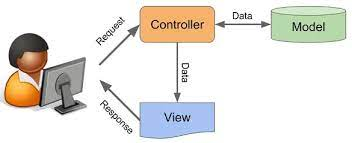
\includegraphics[scale=0.6]{img/mvc.jpg}
\end{figure}

\pagebreak

\section{Implementation}
\begin{justify}
  {\large
  \hspace*{0.5cm} \textcolor{red}{\large D}eveloped using rich client application development tools.
  As well as software grows, complexity increases in parallel.
  This application actually based on JavaFX or a technology which is used to develop more rich desktop apps and mobile embedded systems also.
  Beloved by most of the software engineers and maintained by a large community of developers alongside.\\
  Technologies used here are:
  }
  \begin{enumerate}
    \item[\texttt{Core Java:} ] Used to implement backend logic.
    \item[\texttt{JavaFX:} ] A modern software development technology.
    \item[\texttt{FXML:} ] An extended XML or markup language to give structure of the software.
    \item[\texttt{CSS:} ] Cascading Style Sheet is another ruling language to design the markup or structure like adding padding around the content, give some margin and color or gradients about the component. It makes it looking nice.
    \item[\texttt{Media API:} ] An api for accessing media and its related issues from operating system no matter whatever OS it is, it just creates its own runtime and fetches the files.
    \item[\texttt{Scene Builder:} ] A sophisticated GUI designer developed by Gluon software technologies Inc. Most popular in the community of Java developers.
    \item[\texttt{Maven:} ] Dependency resolver and library bundler for Java. Maintained by Apache Software Foundation. It has huge stock of repositories that enhances developer experience.
  \end{enumerate}
\end{justify}

\section{Result \& Evolution}
\begin{justify}
  {\large
  \hspace*{0.5cm} \textcolor{red}{\large A}fter all, it produces a nice looking media player software.
  More scaled and enhanced, sophisticated and usable, handy interface intended to give better experiences to its end user.
  Code and components structured and organized in such way that is more handy and case easy to debug and inject more feature.
  }
\end{justify}

\pagebreak

\section{Main features}
\begin{justify}
  {\large
  \begin{itemize}
    \item Both audio \& video playing support.
    \item Toggling between fullscreen and minimization mode.
    \item Rollable playlist.
    \item Drag \& Drop accessibility.
    \item UHD, 4K streaming support.
    \item Menubar with huge functionality of interact with the system and optimized shorthands.
    \item High-Level interface includes massive control.
    \item System default interface. No matter whatever users OS is.
    \item Informative media info panel.
    \item Material design included on playlist items.
    \item Don't worry ... use it as you want!
  \end{itemize}
  }
\end{justify}

\section{Future Work}
\begin{justify}
  {\large
  \hspace*{0.5cm} \textcolor{red}{\large D}evelopers behind this have a major goal to employ it as a leading software in the industry level as well as keep it as a open source software under BSMRSTU OPS software license.
  Backends are opened to collaborate. Come up with a handy solution. Add live streaming support with server side programming.
  Robust formation and focus on your media dear client.
  }
\end{justify}

\section{Conclusion}
\begin{justify}
  {\large
  \hspace*{0.5cm} \textcolor{red}{\large A}fter all, successfully developed a JavaFX-based multimedia player that can play audio and video files of various formats.
  We have created a user-friendly and responsive interface that can display and control the media playback.
  Implemented also the features of opening, playing, pausing, stopping, and seeking media files, as well as adjusting the volume, muting, and toggling from full-screen mode to adjusted window.
  We have followed the MVC software pattern to separate the logic, interface, and interaction of this product.
  }
\end{justify}

\pagebreak

\section{Interface Screenshot}
\begin{figure}[!h]
  \centering
  \caption[Interface Initial]{View-1}
  \vspace*{0.1cm}
  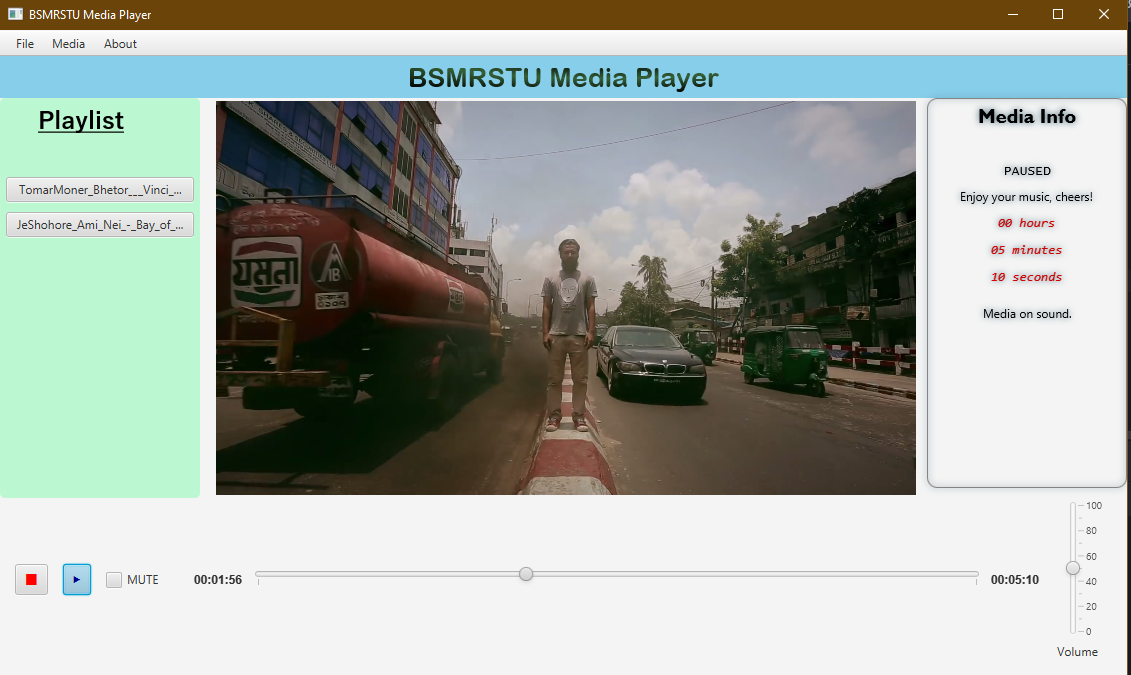
\includegraphics[scale=0.45]{img/view-1.png}
\end{figure}

\begin{figure}[!h]
  \centering
  \caption[Interface Menus]{View-2}
  \vspace*{0.1cm}
  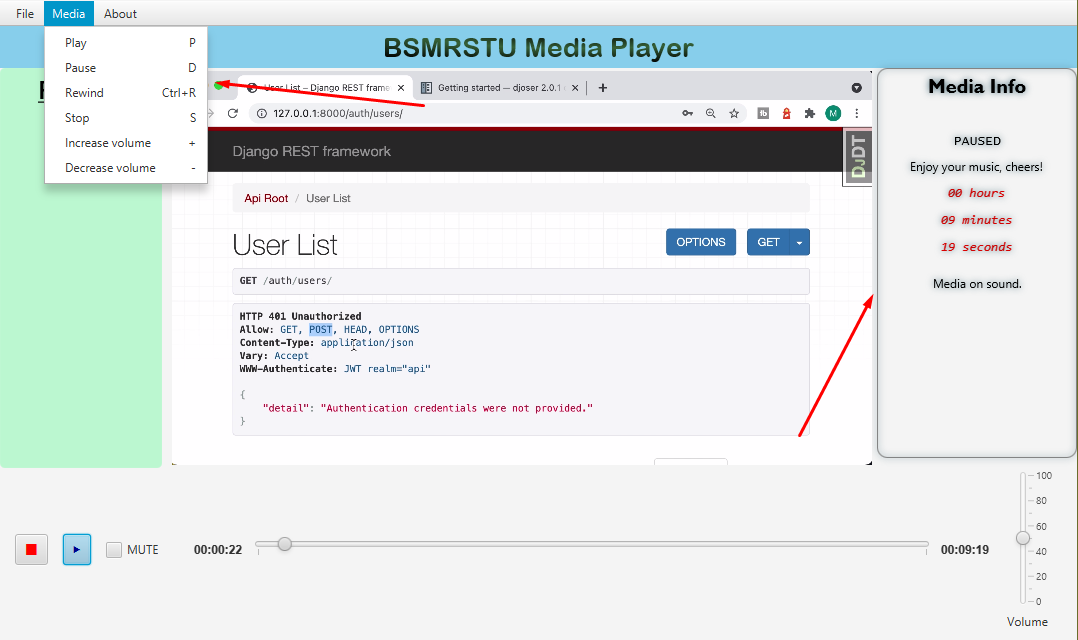
\includegraphics[scale=0.45]{img/view-2.png}
\end{figure}

\section{Code Snapshot}
\begin{lstlisting}[frame = shadowbox, rulesepcolor = \color{blue!80}, language = Java, caption = Snippet from Controller class]
  @Override
  public void initialize(URL location, ResourceBundle resources) {
      System.out.println(getClass().
                        getResource("video.mp4").toString());

      String media_duration = media.getDuration().toString();
      media_view.setMediaPlayer(mediaPlayer);
      total_duration.setText(mediaPlayer.
                            getTotalDuration().toString());
      total_duration.setText(media_duration);

      init_media_player();
      evaluate_duration_slider();
      evaluate_volume_slider();
      evaluate_playlist();
  }

  @FXML
  protected void stop_media(ActionEvent e) {
      if (mediaPlayer != null) {
          if (!mediaPlayer.getStatus().
                              equals(MediaPlayer.Status.STOPPED)) {
              mediaPlayer.stop();
              current_status.setText("STOPPED");
              mediaPlayer.seek(new Duration(0));
              media_view.setOpacity(1);
              duration_slider.adjustValue(0);
          }
      }
//        Platform.exit();
  }

  @FXML
  protected void play_pause_media(ActionEvent e) {
      Status status = mediaPlayer.getStatus();
      if (status == Status.UNKNOWN || status == Status.HALTED) return;
      if (status == Status.PAUSED || status == Status.READY) {
          mediaPlayer.play();
      } else if (status == Status.PLAYING) {
          mediaPlayer.pause();
      }
      alert_message.setText("Enjoy your music, cheers!");
  }
\end{lstlisting}

\vspace*{1.6cm}

\begin{center}
  \textcolor{red}{\LARGE !END\dots}
\end{center}


\end{document}